\section{Wichtige Funktionen}

Viele physikalische und technische Phänomene können analytisch exakt mit Hilfe von mathematischen Funktionen beschrieben werden. Ein bekanntes Beispiel, das häufig im Schulunterricht behandelt wird, ist die Flugbahn eines schräg in die Luft geworfenen Steins. Aber auch ökonomische Beziehungen lassen sich mit Hilfe von Funktionen beschreiben, deren analytische Form sich im Gegensatz zu technischen Anwendungen oft nicht präzise spezifizieren lässt. Besteht zwischen wirtschaftlichen Grundgrößen wie Mengen, Kosten, Preise, Erlöse, Gewinne usw. eine funktionale Beziehung, dann können jedoch oft bestimmte Eigenschaften wie Monotonie oder Extremwertverhalten dieser Funktionen angegeben werden. Die Kenntnis dieser Funktionseigenschaften reicht dann vielfach aus, um daraus ökonomische Folgerungen abzuleiten.

Oft ist allerdings eine ökonomische Variable von mehreren Einflussgrößen abhängig, so dass zu deren Beschreibung eine Funktion mit mehreren unabhängigen Veränderlichen benötigt wird -- beispielsweise kann der Umsatz vom Preis und den getätigten Werbeausgaben abhängen. Häufig ist es jedoch zweckmäßig, nur die Abhängigkeit eines Einflussfaktors isoliert zu betrachten. Die übrigen Einflussgrößen werden dabei als zeitlich unveränderlich, d.\,h. als konstant angenommen. Die funktionale Abhängigkeit der ökonomischen Variablen $y$ von dem isolierten Einflussparameter $x$ wird dann durch die reelle Funktion $y = f(x)$ charakterisiert.

In diesem Abschnitt sollen einige spezielle Funktionen im Detail vorgestellt werden. Die Funktionen können nach ihren Eigenschaften in verschiedene Klassen eingeteilt werden. Die folgende Abbildung zeigt einen Überblick über die \textbf{elementaren Funktionen}.

\begin{center}
  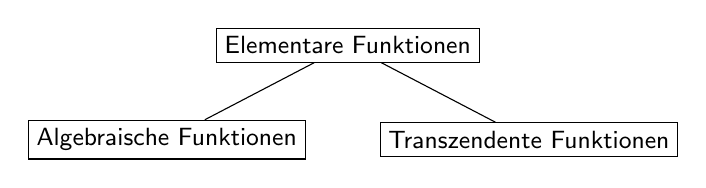
\begin{tikzpicture}[
      box/.style={draw, rectangle, font=\sffamily\small, inner sep=3pt, minimum width=2.6cm},
      level distance=1.2cm, sibling distance=4.6cm]
    \node[box] (r) {Elementare Funktionen}
      child {node[box] {Algebraische Funktionen}}
      child {node[box] {Transzendente Funktionen}};
  \end{tikzpicture}
\end{center}

Die ersten drei Unterabschnitte sind verschiedenen Arten algebraischer Funktionen gewidmet, der letzte beschäftigt sich mit transzendenten Funktionen. Auf die trigonometrischen Funktionen, die speziell transzendente Funktionen sind und eher in technischen Bereichen eine Rolle spielen, wollen wir nicht eingehen.

\subsection{Ganz-rationale Funktionen}

Unter einem \textbf{Polynom in $x$ vom Grad $n$} versteht man einen Ausdruck der Form
\[ y = f(x) = a_n x^n + a_{n-1} x^{n-1} + \ldots + a_1 x + a_0 \]
mit $a_n \neq 0$.

$n$ stellt dabei eine natürliche Zahl dar, und man schreibt $\operatorname{Grad} f(x) = n$ oder $\operatorname{Grad} f = n$. Eine Polynomfunktion wird häufig mit $P(x)$ bezeichnet. Die Zahlen $a_k$ heißen die \textbf{Koeffizienten} des Polynoms $P(x)$. Eine Polynomfunktion wird auch \textbf{ganz-rationale Funktion $n$-ten Grades} genannt.

Die \textbf{linearen Funktionen} sind die einfachsten und wichtigsten Polynome bzw. ganz-rationalen Funktionen. Es handelt sich um Polynome vom Grad 1. Sind $a_1$ und $a_0$ reelle Zahlen, so wird durch
\[ y = f(x) = a_1 x + a_0 \]
eine auf ganz $\mathbb{R}$ definierte Funktion erklärt, deren Graph in der $x,y$-Ebene eine Gerade ist.

Wenn zwei auf einer Geraden liegende Punkte $(x_1;y_1)$ und $(x_2;y_2)$ bekannt sind, können die Koeffizienten $a_0$ und $a_1$ berechnet werden. (Für eine lineare Kostenfunktion wie in Beispiel 1.3.1.1 bedeutet dies: Sind für zwei Anzahlen $x$ die Kosten bekannt, so kann man die ganze Kostenfunktion bestimmen.) Es gilt nämlich:
\begin{align*}
  y_1 &= a_1 x_1 + a_0\\
  y_2 &= a_1 x_2 + a_0
\end{align*}
Daraus erhält man:
\begin{align*}
  a_1 &= \frac{y_2 - y_1}{x_2 - x_1}\\
  a_0 &= \frac{x_2 y_1 - x_1 y_2}{x_2 - x_1}
\end{align*}

\begin{center}
  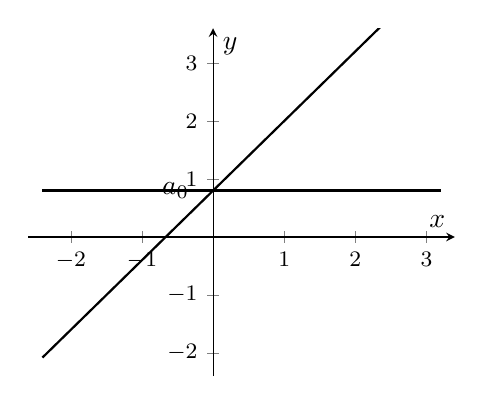
\begin{tikzpicture}
    \begin{axis}[width=7cm, height=6cm, axis lines=middle, xmin=-2.6, xmax=3.4, ymin=-2.4, ymax=3.6,
      xtick={-2,...,3}, ytick={-2,...,3}, xlabel={$x$}, ylabel={$y$}, tick label style={font=\footnotesize}, samples=50]
      \addplot[black, thick, domain=-2.4:3.2] {1.2*x+0.8};
      \addplot[black, thick, domain=-2.4:3.2] {0.8};
      \node[anchor=east] at (axis cs:-0.2,0.8) {$a_0$};
    \end{axis}
  \end{tikzpicture}
\end{center}

Für die Nullstelle $x_0$ der linearen Funktion $f$ folgt aus der Bedingung $f(x_0) = 0$:
\[ x_0 = -\frac{a_0}{a_1} \]
Ist der Koeffizient $a_1 = 0$, so erhält man als Spezialfall der linearen Funktion die konstante Funktion $y = f(x) = a_0$. Ihr Graph ist eine zur $x$-Achse parallele Gerade mit dem $y$-Achsenabschnitt $a_0$. Die Konstante $a_0$ ist dabei eine unveränderliche Größe.

\subsubsection{Beispiele}

\begin{enumerate}[label=\alph*)]
  \item Eine Kostenfunktion $K(x)$ kann in speziellen Fällen linear sein:
    \[ K(x) = K_f + a \cdot x \]
    Die variablen Kosten sind hier proportional zum Output $x$, die Konstante $a$ ist dabei eine positive reelle Zahl.
  \item In der Kinematik ist die gleichförmige Bewegung eine Bewegung mit konstanter Geschwindigkeit $v$. Der zurückgelegte Weg $s$ ist dann eine lineare Funktion der Zeit $t$, der durch die Funktionsgleichung
    \[ s(t) = s_0 + v \cdot t \]
    beschrieben wird. Die Größe $s_0$ gibt dabei die Wegstrecke zu Beginn der Zeitmessung (Anfangswert bei $t = 0$) an.\beispielende
\end{enumerate}

\subsubsection{Übungsaufgabe}

\begin{graukasten}
  Die Gesamtkosten $K(x)$ für die Herstellung von $x$ Einheiten eines gewissen Gutes seien eine lineare Funktion. Aufzeichnungen zeigen, dass einmal 100 Einheiten mit Gesamtkosten von 200\,Euro hergestellt wurden. Ein anderes Mal wurden 150 Einheiten mit Gesamtkosten von 275\,Euro hergestellt. Stellen Sie die lineare Gleichung für die Gesamtkosten $K(x)$ in Abhängigkeit der Anzahl produzierter Einheiten $x$ auf.
\end{graukasten}

Wir kommen nun zu den \textbf{quadratischen Funktionen}. Darunter versteht man Polynome 2. Grades:
\[ y = f(x) = a_2 x^2 + a_1 x + a_0 \]
Ihr Graph ist eine \textbf{Parabel}. Für den Spezialfall $a_1 = 0$ und $a_0 = 0$ liegt der Scheitel der Parabel im Ursprung des Koordinatensystems. Die Graphen der Parabeln $y = f(x) = a_2 x^2$ sind für $|a_2| > 1$ gestreckt und für $|a_2| < 1$ gestaucht. Ihre Scheitel liegen im Ursprung, und sie sind für $a_2 > 0$ nach oben und für $a_2 < 0$ nach unten geöffnet. Der zu $y = f(x) = x^2$ gehörende Graph wird \textbf{Normalparabel} genannt.

Quadratische Funktionen finden sowohl für die Beschreibung einer Vielzahl von technischen Vorgängen an als auch für die Formulierung von wirtschaftlichen Beziehungen Anwendung.

\subsubsection{Beispiele}

\begin{enumerate}[label=\alph*)]
  \item Der freie Fall unter dem Einfluss der konstanten Erdbeschleunigung $g$ stellt bei Vernachlässigung des Reibungswiderstandes der Luft eine gleichmäßig beschleunigte Bewegung dar. Die Abhängigkeit der zurückgelegten Fallstrecke $s$ von der Fallzeit $t$ wird durch eine quadratische Funktion beschrieben:
    \[ s(t) = s_0 + v_0 t + \tfrac{1}{2} g t^2 \]
    Die Größen $s_0$ und $v_0$ sind die Anfangswerte von Weg bzw. Geschwindigkeit zu Beginn der Zeitmessung ($t = 0$).\\
    Für die Koeffizienten gilt: $a_0 = s_0$, $a_1 = v_0$, $a_2 = \tfrac{1}{2} g$.
  \item Die Kostenfunktion $K(x)$, die aus den Fixkosten $K_f$ und den von der erzeugten Menge $x$ abhängigen variablen Kosten $K_v(x)$ zusammengesetzten Gesamtkosten beschreibt, kann auch in Form einer quadratischen Funktion auftreten:
    \[ K(x) = a x^2 + b x + K_f \]
    $a$ und $b$ sind dabei positive Konstanten.\beispielende
\end{enumerate}

Die Nullstellen der quadratischen Funktion
\[ y = f(x) = a_2 x^2 + a_1 x + a_0 \]
ergeben sich als Schnittpunkte der Parabel mit der $x$-Achse. Ist $x_0$ Nullstelle, so gilt:
\[ f(x_0) = a_2 x_0^2 + a_1 x_0 + a_0 = 0 \]
Die Division durch $a_2$ liefert (wenn man $\tfrac{a_1}{a_2}$ durch $p$ und $\tfrac{a_0}{a_2}$ durch $q$ ersetzt) die \textbf{Normalform der quadratischen Gleichung}:
\[ x^2 + p x + q = 0 \]
Die Nullstellen ergeben sich dann zu:
\[ x_{1/2} = -\frac{p}{2} \pm \sqrt{\frac{p^2}{4} - q} \]
(Diese sogenannte \textbf{$p$-$q$-Formel} wurde in Lerneinheit 1 beim Thema »Lösen von Gleichungen« schon einmal behandelt.)

Im nächsten Bild sind zwei Parabeln dargestellt -- eine nach oben geöffnet ($a_2 > 0$), die andere nach unten ($a_2 < 0$). Wie man sieht, schneiden beide zweimal die $x$-Achse -- dies entspricht gerade den Nullstellen gemäß der $p$-$q$-Formel.

\begin{center}
  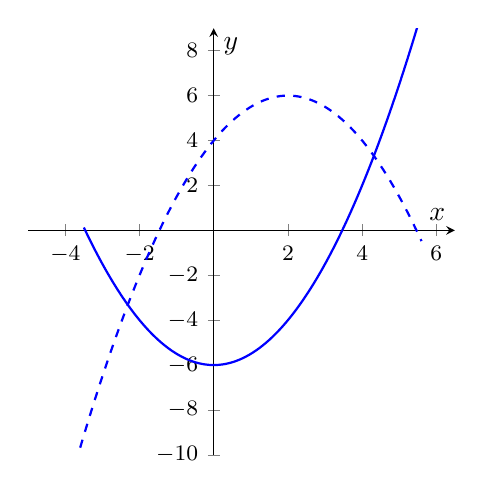
\begin{tikzpicture}
    \begin{axis}[width=7cm, height=7cm, axis lines=middle, xmin=-5, xmax=6.5, ymin=-10, ymax=9,
      xtick={-4,-2,2,4,6}, ytick={-10,-8,...,8}, xlabel={$x$}, ylabel={$y$}, tick label style={font=\footnotesize}, samples=100]
      \addplot[blue, thick, domain=-3.5:5.5] {0.5*x^2-6};
      \addplot[blue, dashed, thick, domain=-3.6:5.6] {-0.5*x^2+2*x+4};
    \end{axis}
  \end{tikzpicture}
\end{center}

Als nächstes wollen wir uns den \textbf{Potenzfunktionen mit natürlichen Exponenten} zuwenden. Ist $n$ eine natürliche Zahl, so ist die durch den Ausdruck
\[ y = f(x) = x^n \]
definierte \textbf{Potenzfunktion} für alle $x \in \mathbb{R}$ erklärt.

Für gerade Exponenten $n$ ist die Potenzfunktion eine \textbf{gerade Funktion}, d.\,h. es gilt:
\[ f(x) = f(-x) \]
Dies bedeutet, dass der Graph einer solchen Funktion spiegelsymmetrisch zur $y$-Achse verläuft. Für den Definitions- und Bildbereich gilt dabei stets $D = \mathbb{R}$ und $B = [0, \infty)$.

\begin{center}
  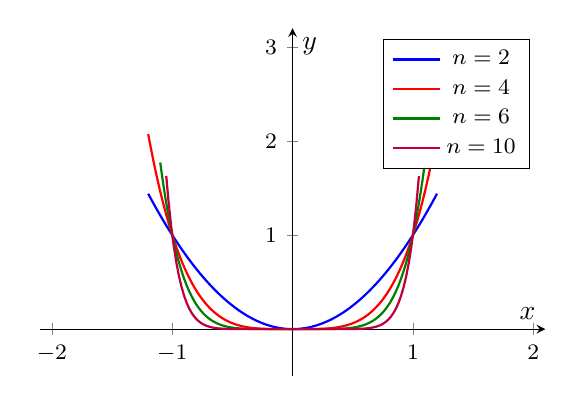
\begin{tikzpicture}
    \begin{axis}[width=8cm, height=6cm, axis lines=middle, xmin=-2.1, xmax=2.1, ymin=-0.5, ymax=3.2,
      xtick={-2,-1,1,2}, ytick={1,2,3}, xlabel={$x$}, ylabel={$y$}, tick label style={font=\footnotesize}, samples=100, legend pos=north east, legend style={font=\footnotesize}]
      \addplot[blue, thick, domain=-1.2:1.2] {x^2};
      \addplot[red, thick, domain=-1.2:1.2] {x^4};
      \addplot[green!50!black, thick, domain=-1.1:1.1] {x^6};
      \addplot[purple, thick, domain=-1.05:1.05] {x^10};
      \legend{$n=2$, $n=4$, $n=6$, $n=10$}
    \end{axis}
  \end{tikzpicture}
\end{center}

Für ungerade Exponenten $n$ ist die Potenzfunktion eine \textbf{ungerade Funktion}, d.\,h. es gilt stets:
\[ f(x) = -f(-x) \]
In diesem Fall verläuft der Graph punktsymmetrisch zum Ursprung des Koordinatensystems. Für den Definitions- und Bildbereich der ungeraden Potenzfunktion erhält man $D = B = \mathbb{R}$.

\begin{center}
  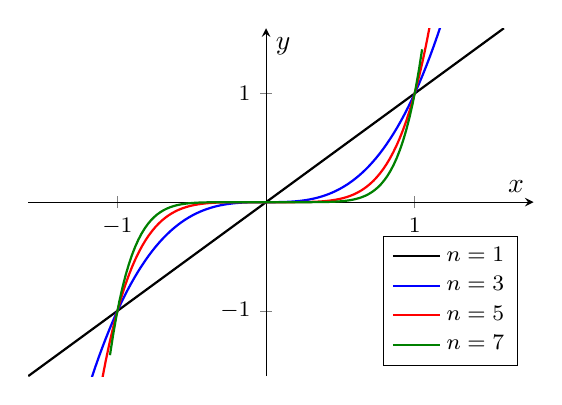
\begin{tikzpicture}
    \begin{axis}[width=8cm, height=6cm, axis lines=middle, xmin=-1.6, xmax=1.8, ymin=-1.6, ymax=1.6,
      xtick={-1,1}, ytick={-1,1}, xlabel={$x$}, ylabel={$y$}, tick label style={font=\footnotesize}, samples=100, legend pos=south east, legend style={font=\footnotesize}]
      \addplot[black, thick, domain=-1.6:1.6] {x};
      \addplot[blue, thick, domain=-1.2:1.2] {x^3};
      \addplot[red, thick, domain=-1.1:1.1] {x^5};
      \addplot[green!50!black, thick, domain=-1.05:1.05] {x^7};
      \legend{$n=1$, $n=3$, $n=5$, $n=7$}
    \end{axis}
  \end{tikzpicture}
\end{center}

Nun kommen wir zum Thema der Polynome zurück, also zu Funktionen der Form
\[ y = f(x) = a_n x^n + a_{n-1} x^{n-1} + \ldots + a_1 x + a_0 . \]
Wir haben gesehen, dass im Falle von Grad 1 (lineare Funktionen) und Grad 2 (quadratische Funktionen) die Nullstellen leicht berechnet werden können. Leider gilt dies ab Grad 3 nicht mehr. Folgendes wurde schon an anderer Stelle gesagt: Für Polynome von Grad 3 und solche von Grad 4 gibt es Formeln (ähnlich der $p$-$q$-Formel für den quadratischen Fall), nach denen die Nullstellen ausgerechnet werden können; diese Formeln sind jedoch recht komplex und nicht gut zu merken. Ab Grad 5 gibt es keine Formeln mehr -- man kann sogar \emph{beweisen}, dass man keine finden kann!

Wie findet man denn nun die Nullstellen eines Polynoms vom Grade 5 oder höher? Zum Glück ist die Lage nicht völlig aussichtslos. Hat man nämlich \emph{eine} Nullstelle gefunden, so kann man immerhin das »Restproblem« auf ein Polynom von kleinerem Grad reduzieren. Dies schreiben wir jetzt genauer hin. Es gilt nämlich der folgende mathematische \textbf{Satz}:

\merkbox{Ist $x_0$ eine Nullstelle des Polynoms $P(x)$ von Grad $n$, d.\,h. Lösung der Polynomgleichung $P(x_0) = 0$, so besitzt das Polynom $P(x)$ eine Faktorzerlegung mit dem Linearfaktor $(x - x_0)$, d.\,h. es gilt
\[ P(x) = (x - x_0) \cdot Q(x) , \]
wobei $Q(x)$ ein Polynom vom Grade $n-1$ ist.}

\subsubsection{Beispiel}

Wir betrachten das Polynom
\[ P(x) = x^3 + x^2 + x - 3 . \]
Wie man durch Einsetzen leicht nachprüft, ist $x_0 = 1$ eine Nullstelle. Folglich muss es ein Polynom $Q(x)$ geben, für das gilt:
\[ P(x) = (x - 1) \cdot Q(x) \]
Dieses Polynom findet man, indem man $P(x)$ durch $(x - 1)$ dividiert (Polynomdivision). Man erhält hier $Q(x) = x^2 + 2x + 3$.\beispielende

Nun kehren wir zur obigen Situation mit gegebenem $P(x)$ und
\[ P(x) = (x - x_0) \cdot Q(x) \]
zurück. Ist $x_1$ eine weitere Nullstelle des Polynoms $P(x)$, so kann man schließen, dass $x_1$ auch eine Nullstelle von $Q(x)$ sein muss. Dies wiederum bedeutet, dass sich das Polynom $Q(x)$ durch Faktorzerlegung in folgender Weise darstellen lässt:
\[ Q(x) = (x - x_1) \cdot Q'(x) \]
Für das Ausgangspolynom $P(x)$ erhält man daraus schließlich:
\[ P(x) = (x - x_0) \cdot (x - x_1) \cdot Q'(x) \]
Kurz gesagt spaltet jede weitere Nullstelle $x_i$ von $P(x)$ einen zusätzlichen Linearfaktor $(x - x_i)$ von $P(x)$ ab. Da das Polynom $P(x)$ vom $n$-ten Grade ist und die Grade der »Restpolynome« $Q(x)$, $Q'(x)$ usw. immer kleiner werden, kann es höchstens $n$ viele Nullstellen besitzen. Denn die Multiplikation von $n$ Linearfaktoren $(x - x_i)$ ergibt gerade ein Polynom $P(x)$ vom Grade $n$.

Dieses Ergebnis kann in folgendem mathematischen \textbf{Satz} zusammengefasst werden:

\merkbox{Ein Polynom $n$-ten Grades besitzt höchstens $n$ verschiedene Nullstellen. Sind $x_1, x_2, \ldots, x_n$ unterschiedliche Nullstellen des Polynoms $P(x)$, dann gilt:
\[ P(x) = a_n x^n + a_{n-1} x^{n-1} + \ldots + a_1 x + a_0 = a_n (x - x_1)(x - x_2) \cdots (x - x_n) \]}

Lässt sich ein gegebener Linearfaktor $(x - x_0)$ mehr als einmal von einem Polynom abspalten, so liegt eine \textbf{mehrfache Nullstelle} vor. $P(x)$ sei ein Polynom $n$-ten Grades. $x_0$ heißt dann eine \textbf{$k$-fache Nullstelle} von $P(x)$, wenn es ein Polynom $S(x)$ vom Grad $n-k$ mit $S(x_0) \neq 0$ gibt, so dass gilt:
\[ P(x) = (x - x_0)^k \cdot S(x) \]

Welche Bedeutung (mehrfache) Nullstellen für die Graphen der Funktionen haben, kann man im folgenden Beispiel sehen.

\subsubsection{Beispiel}

Das Schaubild zeigt Graphen der folgenden drei Funktionen:
\begin{align*}
  f(x) &= (x - 0{,}5)(x - 1{,}5)(x + 0{,}2) = x^3 - 1{,}8x^2 + 0{,}35x + 0{,}15\\
  g(x) &= (x - 1)^2(x + 0{,}2) = x^3 - 1{,}8x^2 + 0{,}6x + 0{,}2\\
  h(x) &= (0{,}3x^2 + 0{,}1)(x + 0{,}2) = 0{,}3x^3 + 0{,}06x^2 + 0{,}1x + 0{,}02
\end{align*}

\begin{center}
  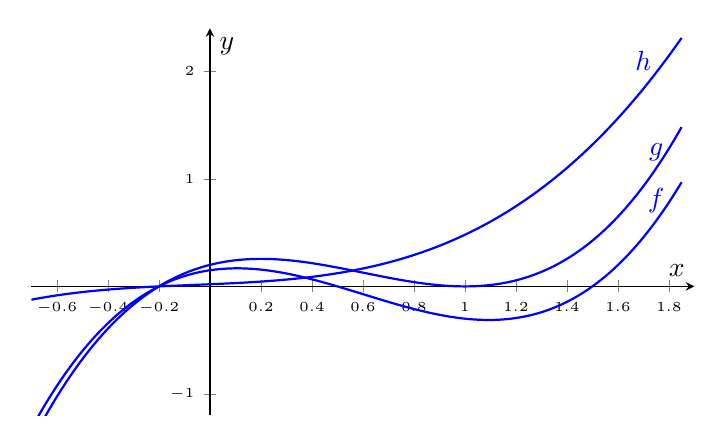
\begin{tikzpicture}
    \begin{axis}[width=10cm, height=6.5cm, axis lines=middle, xmin=-0.7, xmax=1.9, ymin=-1.2, ymax=2.4,
      xtick={-0.6,-0.4,-0.2,0.2,0.4,0.6,0.8,1,1.2,1.4,1.6,1.8}, ytick={-1,1,2}, xlabel={$x$}, ylabel={$y$}, tick label style={font=\tiny}, samples=200]
      \addplot[blue, thick, domain=-0.7:1.85] {(x-0.5)*(x-1.5)*(x+0.2)};
      \addplot[blue, thick, domain=-0.7:1.85] {(x-1)^2*(x+0.2)};
      \addplot[blue, thick, domain=-0.7:1.85] {(0.3*x^2+0.1)*(x+0.2)};
      \node[blue] at (axis cs:1.75,0.8) {$f$};
      \node[blue] at (axis cs:1.75,1.25) {$g$};
      \node[blue] at (axis cs:1.7,2.1) {$h$};
    \end{axis}
  \end{tikzpicture}
\end{center}

$f$ hat die drei Nullstellen $-0{,}2$, $0{,}5$ und $1{,}5$. $g$ hat die zwei Nullstellen $-0{,}2$ und $1$ (doppelt). $h$ hat nur die Nullstelle $-0{,}2$.\beispielende

\subsubsection{Beispiel}

Das Polynom
\[ P(x) = 2x^5 + 12x^4 + 25x^3 + 22x^2 + 12x + 8 \]
besitzt eine dreifache Nullstelle $x_0 = -2$. Es gilt:
\[ P(x) = (x + 2)^3 \cdot (2x^2 + 1) \]
Weitere Nullstellen gibt es nicht.\beispielende

Die letzten Beispiele zeigen, dass das Wort »höchstens« in dem auf der vorigen Seite zitierten mathematischen Satz seine Berechtigung hat: Es können Nullstellen mehrfach vorkommen, und es kann auch sein, dass es weniger als $n$ viele Nullstellen gibt. Mehr kann man sagen, wenn man die \textbf{komplexen Zahlen} mit einbezieht. Für besonders Interessierte ist dazu ein Einschub eingefügt (den nicht alle lesen müssen -- in Lerneinheit 1 wurde darauf bereits kurz eingegangen).

\merkbox{\textbf{Einschub}\\[4pt]
Die Frage nach Existenz und Anzahl der Lösungen einer Polynomgleichung $n$-ten Grades wurde erstmals von C.\,F.\,Gauß 1799 in Form des sogenannten \textbf{Fundamentalsatzes der Algebra} beantwortet:

\medskip
Es seien $a_n$ reelle Zahlen mit $a_n \neq 0$ und $n \geq 1$. Dann besitzt die Polynomgleichung
\[ a_n x^n + a_{n-1} x^{n-1} + \ldots + a_1 x + a_0 = 0 \]
mindestens eine komplexe Lösung. Wird jede $k$-fache Lösung $k$-mal gezählt, so besitzt jede Polynomgleichung $n$-ten Grades im Bereich der komplexen Zahlen genau $n$ Lösungen.

\medskip
In diesem Fundamentalsatz der Algebra sind die komplexen Zahlen angesprochen. An dieser Stelle reicht es zu wissen, dass es sich dabei um eine Erweiterung des Bereiches der reellen Zahlen handelt, die dafür sorgt, dass jedes reelle Polynom -- wie der Fundamentalsatz aussagt -- entsprechend viele Nullstellen besitzt und in Linearfaktoren aufgespalten werden kann.}

\subsubsection{Beispiel}

Wir betrachten das Polynom 2-ten Grades $P(x) = x^2 + 1$ mit den reellen Koeffizienten $a_2 = 1$, $a_1 = 0$ und $a_0 = 1$. Die zugehörige Polynomgleichung lautet:
\[ x^2 + 1 = 0 \]
Diese Gleichung besitzt keine reellen Lösungen. Nach dem Fundamentalsatz besitzt sie jedoch komplexe Lösungen. Dies sind $x_1 = i$ und $x_2 = -i$.\beispielende

Zum Schluss dieses Abschnitts gehen wir kurz darauf ein, wie sich Polynome im Unendlichen verhalten. In Beispiel 1.4.2.3 hatten wir die im Folgenden präsentierte Argumentationsweise schon einmal verwendet. Kurz gesagt:

Das Verhalten im Unendlichen richtet sich nach dem größten Exponenten.

Schauen wir beispielsweise auf die Funktion
\[ y = f(x) = x^3 - 10x^2 + 100x - 50 . \]
Für \emph{sehr große} $x$-Werte (z.\,B. 10.000.000.000) werden die Terme mit $x^2$ und $x$ immer unwichtiger, da der Summand $x^3$ dominierend ist. Daran sieht man: Läuft $x$ gegen $+\infty$, so strebt $f(x)$ ebenfalls gegen $+\infty$ (eben weil dies für $x^3$ so ist) usw.

Im folgenden Bild sind die Funktionen
\[ y = f(x) = 10x^3 - x^2 + 100x - 5 \]
und
\[ y = g(x) = -2x^4 + x^3 + x^2 + 100x + 3000 \]
dargestellt. Man sieht, dass sich $f(x)$ im Unendlichen wie »$10x^3$« und $g(x)$ wie »$-2x^4$« verhält.

\begin{center}
  \begin{tikzpicture}
    \begin{axis}[width=10cm, height=7cm, axis lines=left, xmin=-22, xmax=22, ymin=-350000, ymax=150000,
      xtick={-20,-15,...,20}, ytick={-300000,-200000,-100000,0,100000}, xlabel={$x$}, tick label style={font=\tiny},
      scaled y ticks=false, samples=200, yticklabels={$-300.000$,$-200.000$,$-100.000$,$0$,$100.000$}]
      \addplot[black, thick, domain=-22:22, restrict y to domain=-350000:150000] {10*x^3-x^2+100*x-5};
      \addplot[black, thick, domain=-22:22, restrict y to domain=-350000:150000] {-2*x^4+x^3+x^2+100*x+3000};
    \end{axis}
  \end{tikzpicture}
\end{center}

\subsubsection{Übungsaufgabe}

\begin{graukasten}
  Bestimmen Sie alle Nullstellen des Polynoms $P(x) = x^3 - 3x - 2$.
\end{graukasten}

\subsection{Gebrochen-rationale Funktionen}

Eine Funktion der Form
\[ y = f(x) = \frac{a_n x^n + a_{n-1} x^{n-1} + \ldots + a_1 x + a_0}{b_m x^m + b_{m-1} x^{m-1} + \ldots + b_1 x + b_0} = \frac{Z(x)}{N(x)} \]
mit $a_i$ und $b_j \in \mathbb{R}$ und $m \geq 1$ heißt \textbf{gebrochen-rationale Funktion}. Sie ist definiert für alle $x$ mit $N(x) \neq 0$.

Die Funktion heißt \textbf{echt gebrochen}, wenn der Grad $n$ des Zählerpolynoms kleiner als der Grad $m$ des Nennerpolynoms ist, andernfalls heißt sie \textbf{unecht gebrochen}.

Jede unecht gebrochen-rationale Funktion kann durch Polynomdivision in die Summe einer ganz-rationalen Funktion und einer echt gebrochen-rationalen Funktion zerlegt werden.

\subsubsection{Beispiele}

\begin{enumerate}[label=\alph*)]
  \item Die Funktion
    \[ y = f(x) = \frac{5x^2 + 4x + 3}{x^3 - x + 1} \]
    ist eine echt gebrochen-rationale Funktion.
  \item Die Funktion
    \[ y = f(x) = \frac{2x^3 + 2x - 3}{x^3 + 5x^2} \]
    ist eine unecht gebrochen-rationale Funktion. Durch Polynomdivision findet man heraus:
    \[ f(x) = 2 + \frac{-10x^2 + 2x - 3}{x^3 + 5x^2} \]
  \item Die Funktion
    \[ y = f(x) = \frac{x^3 - 3x + 5}{x - 2} \]
    ist eine unecht gebrochen-rationale Funktion. Sie lässt sich als Summe eines ganz-rationalen Polynoms und einer echt gebrochen-rationalen Funktion darstellen, wie man ebenfalls durch Polynomdivision herausfindet:
    \[ y = f(x) = \frac{x^3 - 3x + 5}{x - 2} = x^2 + 2x + 1 + \frac{7}{x - 2}\beispielende \]
\end{enumerate}

Die \textbf{Nullstellen} einer gebrochen-rationalen Funktion ergeben sich als diejenigen Nullstellen des Zählerpolynoms $Z(x)$, für die die Funktion definiert, d.\,h. das Nennerpolynom nicht Null ist. Unter den Werten $x_0$, für die die Funktion \emph{nicht} definiert ist (wegen $N(x_0) = 0$), sind diejenigen noch einmal von besonderem Interesse, für die auch $Z(x_0) = 0$ gilt -- es handelt sich um sogenannte \textbf{Lücken}. Wir gehen nicht weiter darauf ein.

Eine besondere Rolle unter den gebrochen-rationalen Funktionen spielen die Potenzfunktionen mit negativem ganzzahligen Exponenten. Die Potenzfunktion $y = f(x) = x^{-n}$ mit $n \in \mathbb{N}$ kann als reziproke Funktion der Potenzfunktion $g(x) = x^n$ aufgefasst werden:
\[ f(x) = \frac{1}{g(x)} = \frac{1}{x^n} = x^{-n} \]

\subsection{Irrationale Funktionen}

Bei \textbf{irrationalen Funktionen} kommt bei der analytischen Zuordnungsvorschrift zu den arithmetischen Grundrechenoperationen, die zu Polynomen und Brüchen von Polynomen führen, das Wurzelziehen hinzu. Die irrationalen Funktionen bilden zusammen mit den ganz-rationalen und den gebrochen-rationalen Funktionen die \textbf{algebraischen Funktionen}.

\subsubsection{Beispiel}

Die Funktion $y = f(x) = +\sqrt{1 - x^2}$ ist eine irrationale Funktion. Ihr Graph beschreibt den oberen Halbkreis um den Ursprung des Koordinatensystems mit dem Radius $r = 1$.\beispielende

Potenzfunktionen mit gebrochenem Exponenten $r = \tfrac{m}{n}$ mit teilerfremden Zahlen $m \in \mathbb{Z}$ und $n \in \mathbb{N}$ heißen \textbf{Wurzelfunktionen}. Man hat dann:
\[ y = f(x) = x^r = x^{\frac{m}{n}} = \sqrt[n]{x^m} \]
Definitions- und Bildbereich der Wurzelfunktionen werden durch den Exponenten $r = \tfrac{m}{n}$ der Potenzfunktion bestimmt.

Ist der Wurzelexponent $n$ gerade, so existieren nur für positive Elemente $x$ des Definitionsbereiches reelle $y$-Werte des Bildbereichs, da die negativen Zahlen bei geradzahligem Wurzelexponenten keine reellen Wurzeln besitzen. Diese Einschränkung gilt nicht für Funktionen mit ungeraden Wurzelexponenten $n$.

\subsubsection{Beispiele}

\begin{enumerate}[label=\alph*)]
  \item Die Funktion $y = f(x) = x^{\frac{1}{2}} = \sqrt{x}$ mit $m = 1$ und $n = 2$ ist nur für positive $x$-Werte ($x \geq 0$) definiert.
  \item Die Funktion $y = f(x) = x^{\frac{1}{3}} = \sqrt[3]{x}$ mit $m = 1$ und $n = 3$ ist für alle $x \in \mathbb{R}$ erklärt. So ergibt sich z.\,B. für $x = -8$ der Funktionswert $y = \sqrt[3]{-8} = -2$. Der Graph dieser Funktion ist in der folgenden Abbildung dargestellt.\beispielende
\end{enumerate}

\begin{center}
  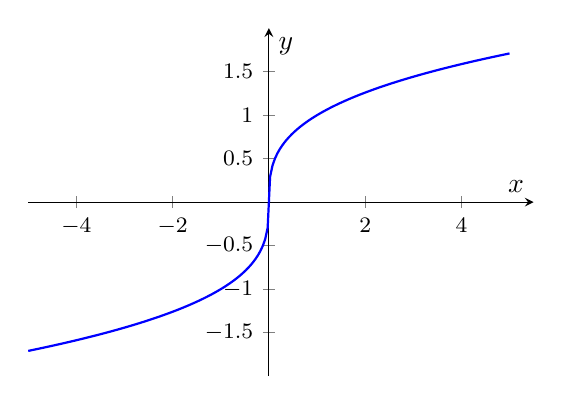
\begin{tikzpicture}
    \begin{axis}[width=8cm, height=6cm, axis lines=middle, xmin=-5, xmax=5.5, ymin=-2, ymax=2, xtick={-4,-2,2,4}, ytick={-1.5,-1,-0.5,0.5,1,1.5}, xlabel={$x$}, ylabel={$y$}, tick label style={font=\footnotesize}, samples=200, domain=-5:5, restrict y to domain=-2:2]
      \addplot[blue, thick] {sign(x)*abs(x)^(1/3)};
    \end{axis}
  \end{tikzpicture}
\end{center}

Für den Definitionsbereich von Wurzelfunktionen gilt bei ungeradem Wurzelexponenten $n$: $D = \mathbb{R}$. Für geraden Wurzelexponenten besitzen Wurzelfunktionen den Definitionsbereich $D = [0, \infty)$.

Für den Spezialfall $m = 1$ erhält man die Wurzelfunktion
\[ y = f(x) = x^{\frac{1}{n}} = \sqrt[n]{x} . \]
Sie stellt die Umkehrfunktion der Potenzfunktion $y = f(x) = x^n$ dar.

Die allgemeine Potenzfunktion $y = f(x) = x^r$ ist für positive Exponenten ($r > 0$) streng monoton wachsend, für negative Exponenten ($r < 0$) streng monoton fallend. Ihre Umkehrfunktion $f^{-1}$ ist wieder eine Potenzfunktion. Es gilt:
\begin{align*}
  y &= f(x) = x^r\\
  x &= \sqrt[r]{y} = y^{\frac{1}{r}}\\
  y &= f^{-1}(x) = x^{\frac{1}{r}}
\end{align*}

\subsubsection{Beispiel}

Die folgende Abbildung zeigt verschiedene Graphen der allgemeinen Potenzfunktion $y = f(x) = x^r$ mit den Exponenten $r = \tfrac{3}{2}$, $r = \tfrac{1}{2}$ und $r = -\tfrac{1}{2}$.

\begin{center}
  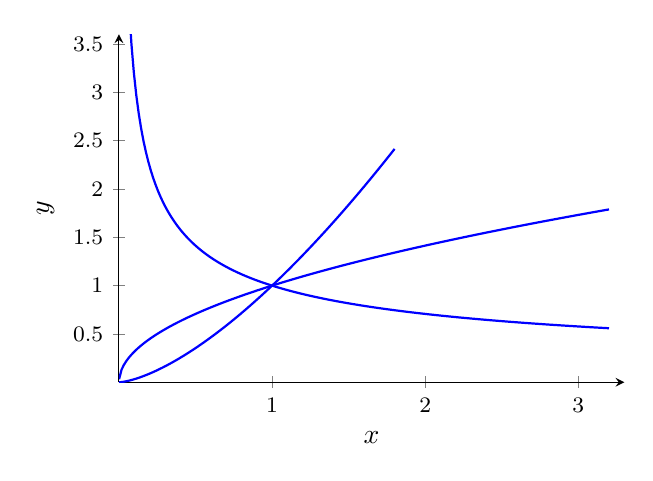
\begin{tikzpicture}
    \begin{axis}[width=8cm, height=6cm, axis lines=left, xmin=0, xmax=3.3, ymin=0, ymax=3.6,
      xtick={1,2,3}, ytick={0.5,1,...,3.5}, xlabel={$x$}, ylabel={$y$}, tick label style={font=\footnotesize}, samples=200]
      \addplot[blue, thick, domain=0.001:1.8] {x^(3/2)};
      \addplot[blue, thick, domain=0.001:3.2] {x^(1/2)};
      \addplot[blue, thick, domain=0.05:3.2] {x^(-1/2)};
    \end{axis}
  \end{tikzpicture}
\end{center}\beispielende

\subsection{Transzendente Funktionen}

Von den transzendenten Funktionen behandeln wir nur die \textbf{Exponentialfunktionen} und die \textbf{Logarithmusfunktionen}. (Auf die für viele Anwendungen ebenfalls wichtigen \textbf{trigonometrischen Funktionen} wie Sinus, Kosinus etc. gehen wir nicht ein.)

Es sei $a > 0$. Die durch die Funktionsgleichung $y = f(x) = a^x$ für alle reellen $x$ erklärte Funktion heißt \textbf{Exponentialfunktion zur Basis $a$}.

Man beachte: Im Gegensatz zu den bisher von uns betrachteten Funktionen (wie z.\,B. Polynome) steht das $x$ hier »oben«.

\subsubsection{Beispiel}

Angenommen, ein Auto hat heute einen Wert von 20000\,€. Welchen Wert hat es in 6 Jahren, wenn man annimmt, dass der Wert jedes Jahr
\begin{enumerate}[label=\alph*)]
  \item um 10\,\% des heutigen Wertes abnimmt?
  \item um 10\,\% des jeweiligen Wertes abnimmt?
\end{enumerate}

\begin{enumerate}[label=\alph*)]
  \item Für den Wert nach $t$ Jahren hat man hier die lineare Funktion
    \[ w(t) = 20000 - 2000 \cdot t . \]
    Nach 6 Jahren ist also $w(6) = 8000$.
  \item Man muss sich hier klarmachen, dass eine Abnahme einer Größe um 10\,\% die Multiplikation mit 0{,}9 bedeutet. Dann ist klar, dass die Fragestellung auf die Berechnung von
    \[ 20000 \cdot 0{,}9^6 \]
    hinausläuft, was ca. 10628{,}82\,€ ergibt.
    Man hat hier eine Exponentialfunktion: Will man den Wert des Autos nach $t$ Jahren wissen, so ist die Antwort
    \[ w(t) = 20000 \cdot 0{,}9^t . \]\beispielende
\end{enumerate}

Für das Monotonieverhalten der allgemeinen Exponentialfunktion gilt (siehe das folgende Bild):
\[ y = f(x) = a^x \text{ ist} \]
\begin{itemize}
  \item streng monoton wachsend für $a > 1$,
  \item streng monoton fallend für $0 < a < 1$,
  \item konstant für $a = 1$.
\end{itemize}

\begin{center}
  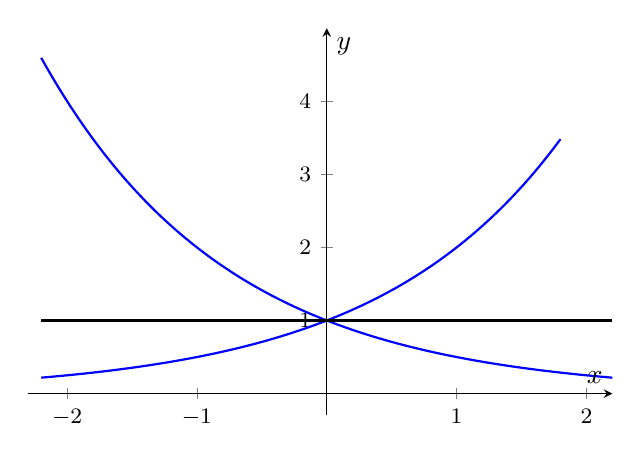
\begin{tikzpicture}
    \begin{axis}[width=9cm, height=6.5cm, axis lines=middle, xmin=-2.3, xmax=2.2, ymin=-0.3, ymax=5,
      xtick={-2,-1,1,2}, ytick={1,2,3,4}, xlabel={$x$}, ylabel={$y$}, tick label style={font=\footnotesize}, samples=100]
      \addplot[blue, thick, domain=-2.2:1.8] {2^x};
      \addplot[blue, thick, domain=-2.2:2.2] {0.5^x};
      \addplot[black, thick, domain=-2.2:2.2] {1};
    \end{axis}
  \end{tikzpicture}
\end{center}

Für das Verhalten im Unendlichen gilt:
\begin{align*}
  a^x &\rightarrow \infty \quad \text{für } x \rightarrow \infty \text{ und } a > 1\\
  a^x &\rightarrow 0 \quad \text{für } x \rightarrow -\infty \text{ und } a > 1\\
  a^x &\rightarrow 0 \quad \text{für } x \rightarrow \infty \text{ und } 0 < a < 1\\
  a^x &\rightarrow \infty \quad \text{für } x \rightarrow -\infty \text{ und } 0 < a < 1
\end{align*}

Exponentialfunktionen besitzen keine reellen Nullstellen, denn für alle $x \in \mathbb{R}$ gilt $a^x > 0$. Für die Funktionswerte an den Stellen $x = 0$, $x = 1$ und $x = -1$ erhält man
\[ a^0 = 1 , \quad a^1 = a \quad \text{und} \quad a^{-1} = \tfrac{1}{a} . \]

\subsubsection{Beispiel}

Die Graphen der Exponentialfunktionen $y = f(x) = 10^x$, $y = f(x) = 2^x$ und $y = f(x) = \left(\tfrac{1}{2}\right)^x$ sind in der folgenden Abbildung dargestellt.

\begin{center}
  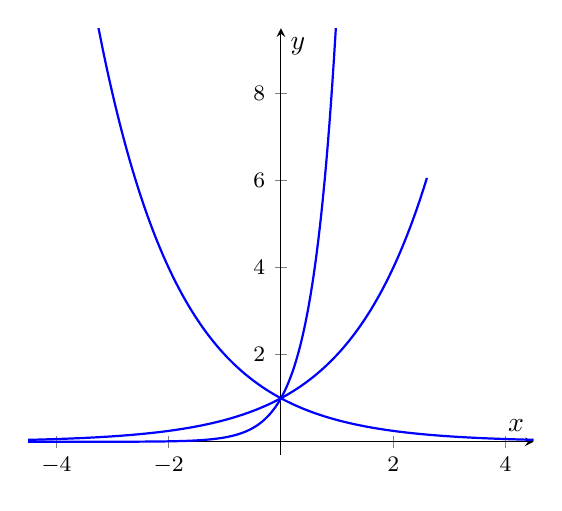
\begin{tikzpicture}
    \begin{axis}[width=8cm, height=7cm, axis lines=middle, xmin=-4.5, xmax=4.5, ymin=-0.3, ymax=9.5,
      xtick={-4,-2,2,4}, ytick={2,4,6,8}, xlabel={$x$}, ylabel={$y$}, tick label style={font=\footnotesize}, samples=200]
      \addplot[blue, thick, domain=-4.5:1.0] {10^x};
      \addplot[blue, thick, domain=-4.5:2.6] {2^x};
      \addplot[blue, thick, domain=-4.5:4.5] {0.5^x};
    \end{axis}
  \end{tikzpicture}
\end{center}\beispielende

Im Exponenten einer Exponentialfunktion (also »oben«) können selbstverständlich auch komplexere Ausdrücke eingesetzt werden, m.\,a.\,W. werden auch $y = f(x) = 2^{5x}$ oder $y = f(x) = 3{,}1^{x^2 - 3}$ als Exponentialfunktionen bezeichnet.

Von besonderer mathematischer Bedeutung ist die spezielle Exponentialfunktion mit der Basis $a = e$:
\[ y = f(x) = e^x \]
Die Eulersche Zahl $e$ bildet die Basis dieser als \textbf{$e$-Funktion} bezeichneten Exponentialfunktion. Wie schon in Lerneinheit 1 erwähnt, ist $e$ eine transzendente Zahl. Insbesondere beinhaltet dies, dass $e$ nur beliebig genau, nicht jedoch exakt angegebbar ist. Der Zahlenwert ist
\[ e = 2{,}71828\ldots \]
Die $e$-Funktion wird auch als \textbf{Wachstumsfunktion} bezeichnet. Für das Wachstumsverhalten der $e$-Funktion gilt (wie für alle Exponentialfunktionen $y = f(x) = a^x$ mit $a > 1$):
\merkbox{Die Funktion $y = f(x) = e^x$ steigt »schneller« an als jede Potenzfunktion der Form $y = f(x) = x^n$.}

Interessant ist noch anzumerken, dass Exponentialfunktionen zu einer Basis $a$ stets in Exponentialfunktionen zu einer Basis $b$ umgewandelt werden können.

\subsubsection{Beispiel}

Alle Exponentialfunktionen sind als $e$-Funktion darstellbar. Als Beispiel soll die Exponentialfunktion $y = f(x) = 5 \cdot 2^x$ als $e$-Funktion dargestellt werden. Wegen
\[ 2 = e^{\ln 2} \]
kann man nämlich schreiben
\[ 5 \cdot 2^x = 5 \cdot \left(e^{\ln 2}\right)^x = 5 \cdot e^{\ln 2 \cdot x} , \]
man hat also
\[ y = f(x) = 5 \cdot e^{\ln 2 \cdot x} .\beispielende \]

Die Funktion
\[ y = f(x) = e^{-x} = \frac{1}{e^x} \]
wird als \textbf{reziproke $e$-Funktion} oder auch \textbf{Dämpfungsfunktion} bezeichnet (vgl. dazu die folgende Abbildung).

\begin{center}
  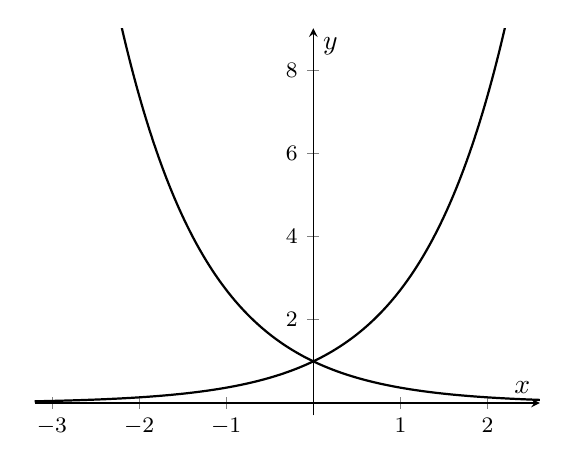
\begin{tikzpicture}
    \begin{axis}[width=8cm, height=6.5cm, axis lines=middle, xmin=-3.2, xmax=2.6, ymin=-0.3, ymax=9,
      xtick={-3,-2,-1,1,2}, ytick={2,4,6,8}, xlabel={$x$}, ylabel={$y$}, tick label style={font=\footnotesize}, samples=200]
      \addplot[black, thick, domain=-3.2:2.6] {exp(x)};
      \addplot[black, thick, domain=-3.2:2.6] {exp(-x)};
    \end{axis}
  \end{tikzpicture}
\end{center}

Die praktische Bedeutung der $e$-Funktion soll durch ein weiteres Beispiel erläutert werden.

\subsubsection{Beispiel}

Unter Berücksichtigung von Zinseszinsen ist ein Betrag von $K_0$ Geldeinheiten, der bei einem Zinsfuß von $p\,\%$ angelegt wird, nach Ablauf eines Jahres auf den Betrag
\[ K_0 \cdot \left(1 + \frac{p}{100}\right) \]
angewachsen. Nach Ablauf von $t$ Jahren beträgt das Kapital
\[ K(t) = K_0 \cdot \left(1 + \frac{p}{100}\right)^t . \]
Die Zinsen wurden dabei einmal jährlich dem Kapital zugeschlagen und von da ab mit verzinst. Werden die Zinsen dagegen halbjährlich zugeschlagen und mit verzinst, so wird üblicherweise der Zinssatz halbiert; damit ergibt sich das Kapital $K(t)$ zu:
\[ K(t) = K_0 \cdot \left(1 + \frac{p}{2 \cdot 100}\right)^{2t} \]
Bei $\tfrac{1}{n}$-jährlicher Verzinsung werden die Zinsen $n$-mal pro Jahr dem jeweiligen Kapital zugeschlagen und mit verzinst. Nach $t$ Jahren ergibt sich dann das Kapital
\[ K(t) = K_0 \cdot \left(1 + \frac{p}{n \cdot 100}\right)^{nt} . \]
Mit wachsendem $n$ werden die »Zinszeiträume« immer kleiner, und im Grenzübergang $n \rightarrow \infty$ folgt:
\[ K(t) \rightarrow K_0 \cdot e^{\left(\frac{p}{100}\right) t} \]
(Da wir Grenzwerte solcher »Folgen« nicht behandelt haben, können wir dieses Ergebnis hier nicht begründen.)
Diese Form der Verzinsung heißt \textbf{stetige Verzinsung}. (Ein derartiger Funktionsverlauf ist auch für alle organischen Wachstumsprozesse mit stetigem Wachstum und konstanter Wachstumsrate charakteristisch, z.\,B. die Holzzunahme einer aufgeforsteten Waldfläche.)\beispielende

\structhead{Logarithmusfunktionen}

Jetzt kommen wir zu den \textbf{Logarithmusfunktionen}.

Eine Funktion $y = f(x) = \log_a x$ mit $a > 0$ und $a \neq 1$ heißt \textbf{Logarithmusfunktion}. Die reelle Zahl $a$ heißt \textbf{Basis} der Logarithmusfunktion.

Die Logarithmusfunktion $y = f(x) = \log_a x$ ist die Umkehrfunktion der Exponentialfunktion $y = f(x) = a^x$. Umgekehrt ist die Exponentialfunktion die inverse Funktion zur Logarithmusfunktion. Es gilt nämlich:
\[ y = a^x \text{ ist gleichbedeutend mit } x = \log_a y . \]
Vertauschen der Variablen $x$ und $y$ liefert somit als inverse Funktion zur Exponentialfunktion
\[ y = \log_a x . \]

\begin{center}
  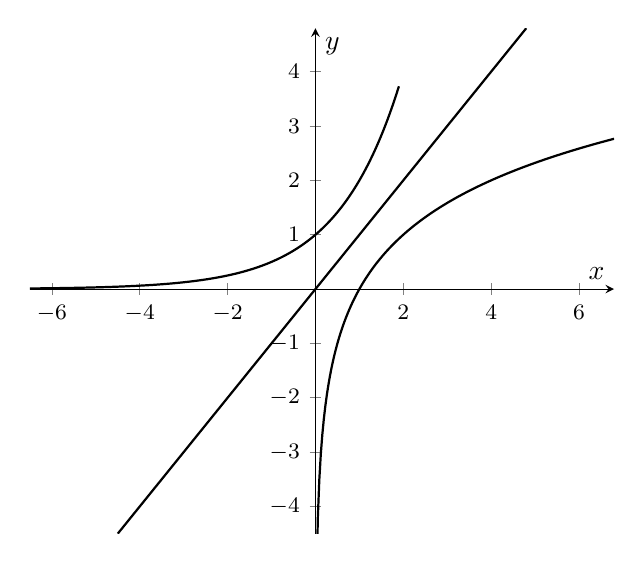
\begin{tikzpicture}
    \begin{axis}[width=9cm, height=8cm, axis lines=middle, xmin=-6.5, xmax=6.8, ymin=-4.5, ymax=4.8,
      xtick={-6,-4,-2,2,4,6}, ytick={-4,...,4}, xlabel={$x$}, ylabel={$y$}, tick label style={font=\footnotesize}, samples=200]
      \addplot[black, thick, domain=-6.5:1.9] {2^x};
      \addplot[black, thick, domain=0.02:6.8] {ln(x)/ln(2)};
      \addplot[black, thick, domain=-4.5:4.8] {x};
    \end{axis}
  \end{tikzpicture}
\end{center}

Der Graph der logarithmischen Funktion ergibt sich aus dem Graphen der Exponentialfunktion gleicher Basis durch Spiegelung an der Winkelhalbierenden $y = x$.

Wegen $a^0 = 1$ und $a^1 = a$ besitzt die Logarithmusfunktion $y = f(x) = \log_a x$ für alle Basen $a > 0$ die speziellen Funktionswerte
\[ f(1) = \log_a 1 = 0 \]
und
\[ f(a) = \log_a a = 1 . \]

Für die Logarithmusfunktionen mit den Basen $a = 10$, $a = e$ und $a = 2$ gelten folgende abkürzende Schreibweisen:
\begin{align*}
  y = f(x) &= \log_{10} x = \lg x\\
  y = f(x) &= \log_e x = \ln x\\
  y = f(x) &= \log_2 x = \operatorname{lb} x
\end{align*}

\begin{center}
  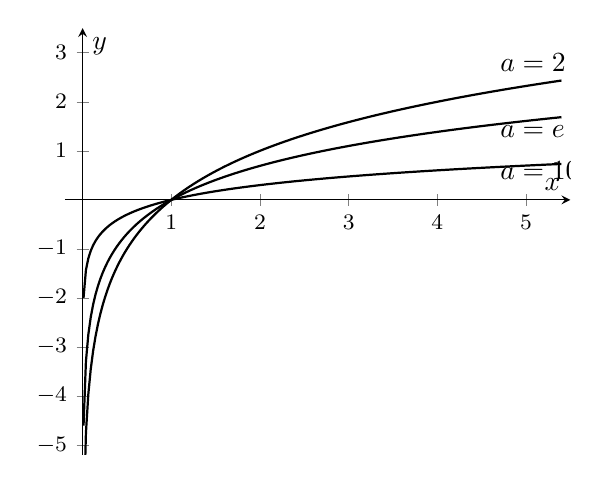
\begin{tikzpicture}
    \begin{axis}[width=8cm, height=7cm, axis lines=middle, xmin=-0.2, xmax=5.5, ymin=-5.2, ymax=3.5,
      xtick={1,2,3,4,5}, ytick={-5,...,3}, xlabel={$x$}, ylabel={$y$}, tick label style={font=\footnotesize}, samples=200, domain=0.01:5.4]
      \addplot[black, thick] {ln(x)/ln(2)};
      \addplot[black, thick] {ln(x)};
      \addplot[black, thick] {ln(x)/ln(10)};
      \node[anchor=west] at (axis cs:4.6,2.8) {$a = 2$};
      \node[anchor=west] at (axis cs:4.6,1.4) {$a = e$};
      \node[anchor=west] at (axis cs:4.6,0.6) {$a = 10$};
    \end{axis}
  \end{tikzpicture}
\end{center}

Die Logarithmusfunktionen sind für Basen $a > 1$ streng monoton wachsend und für Basen $0 < a < 1$ streng monoton fallend. Eine Logarithmusfunktion ist nur für positive $x$-Werte erklärt, d.\,h. für ihren Definitionsbereich gilt $D = (0, \infty)$.

In der folgenden Abbildung ist die Logarithmusfunktion $y = f(x) = \log_{\frac{1}{2}} x$ mit der Basis $a = \tfrac{1}{2}$ gezeigt. Gleichzeitig ist auch die zugehörige Umkehrfunktion
\[ y = f(x) = \left(\tfrac{1}{2}\right)^x \]
dargestellt.

\begin{center}
  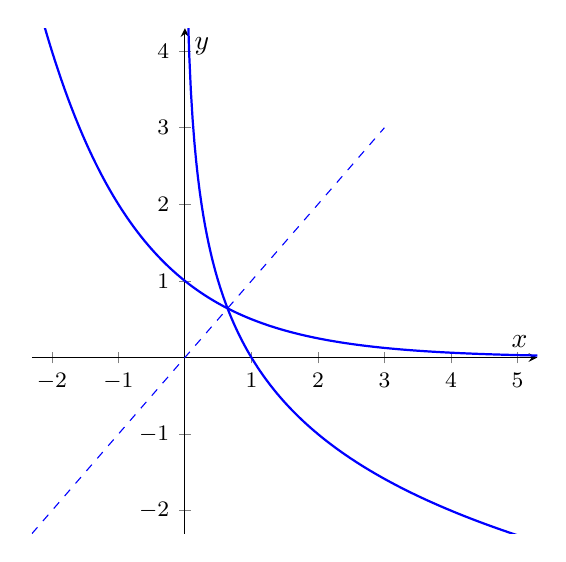
\begin{tikzpicture}
    \begin{axis}[width=8cm, height=8cm, axis lines=middle, xmin=-2.3, xmax=5.3, ymin=-2.3, ymax=4.3,
      xtick={-2,-1,1,2,3,4,5}, ytick={-2,-1,1,2,3,4}, xlabel={$x$}, ylabel={$y$}, tick label style={font=\footnotesize}, samples=200]
      \addplot[blue, thick, domain=-2.3:5.3] {0.5^x};
      \addplot[blue, thick, domain=0.01:5.3] {ln(x)/ln(0.5)};
      \addplot[blue, dashed, domain=-2.3:3] {x};
    \end{axis}
  \end{tikzpicture}
\end{center}

Sind die Logarithmen für eine Basis $a$ bekannt, so folgt für die Logarithmen für eine andere Basis $b$ ($b > 0$ und $b \neq 1$):
\[ \log_b x = \frac{\log_a x}{\log_a b} \]
$k = \dfrac{1}{\log_a b}$ ist eine Konstante, man hat damit:
\[ y = f(x) = \log_b x = k \cdot \log_a x \]
Mit anderen Worten sind die Logarithmusfunktionen mit verschiedenen Basen zueinander proportional.

\subsubsection{Übungsaufgabe}

\begin{graukasten}
  Bestimmen Sie die Nullstellen der Funktion $y = f(x) = \ln(x^2 - 3)$.
\end{graukasten}
